% Simple schematic of the instance segmentation pipelines (RT-DETR and Mask R-CNN) with a shared encoder.
\begingroup
% Shared visual language for the three segmentation-method diagrams.
\tikzset{
    box/.style={draw, rounded corners=2pt, align=center, font=\small,
        text width=44mm, minimum height=9mm, inner sep=4pt, line width=0.5pt},
    process/.style={box, fill=gray!7},
    model/.style={box, very thick, fill=blue!5},
    output/.style={box, dashed},
    supervision/.style={box, densely dashed, fill=gray!7},
    link/.style={->, semithick},
    traininglink/.style={link, densely dashed}
}

\usetikzlibrary{calc}
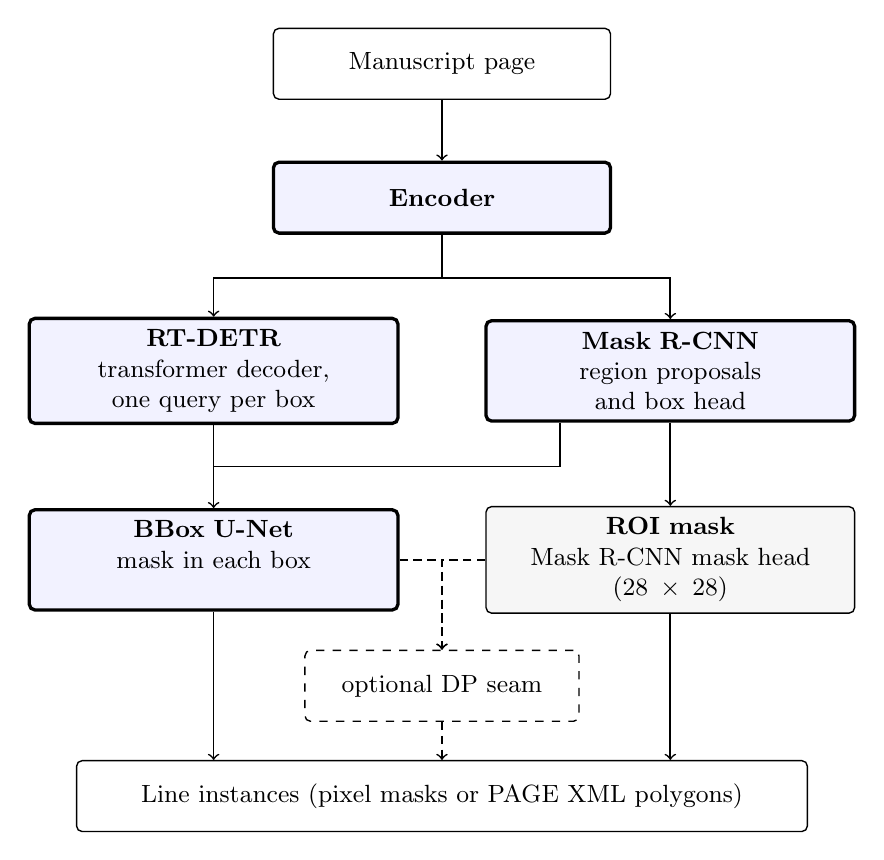
\begin{tikzpicture}
    \node[box, text width=40mm] (page) at (0,0) {Manuscript page};
    \node[model, text width=40mm] (enc) at (0,-1.7) {\textbf{Encoder}};
    \node[model, text width=44mm] (rtdetr) at (-2.9,-3.9) {\textbf{RT-DETR}\\transformer decoder,\\one query per box};
    \node[model, text width=44mm] (mrcnn) at (2.9,-3.9) {\textbf{Mask R-CNN}\\region proposals\\and box head};
    \node[model, text width=44mm] (crop) at (-2.9,-6.3) {\textbf{BBox U-Net}\\mask in each box\\\phantom{x}};
    \node[process, text width=44mm] (roi) at (2.9,-6.3) {\textbf{ROI mask}\\Mask R-CNN mask head\\(\(28\times28\))};
    \node[output, text width=32mm] (seam) at (0,-7.9) {optional DP seam};
    \node[box, text width=90mm] (lines) at (0,-9.3) {Line instances (pixel masks or PAGE XML polygons)};
    \draw[link] (page) -- (enc);
    % fork from the shared encoder to both detectors
    \coordinate (fork) at ($(enc.south)+(0,-0.55)$);
    \draw[semithick] (enc.south) -- (fork);
    \draw[link] (fork) -| (rtdetr.north);
    \draw[link] (fork) -| (mrcnn.north);
    \draw[link] (rtdetr.south) -- (rtdetr.south |- crop.north);
    % Mask R-CNN boxes join the RT-DETR -> BBox U-Net arrow
    \coordinate (mstart) at ($(mrcnn.south)+(-1.4,0)$);
    \coordinate (join) at ($(rtdetr.south)!0.5!(rtdetr.south |- crop.north)$);
    \draw[semithick] (mstart) |- (join);
    \draw[link] (mrcnn.south) -- (mrcnn.south |- roi.north);
    \draw[traininglink] (crop.east) -| (seam.north);
    \draw[traininglink] (roi.west) -| (seam.north);
    \draw[traininglink] (seam.south) -- (lines.north);
    \draw[link] (crop.south) -- (crop.south |- lines.north);
    \draw[link] (roi.south) -- (roi.south |- lines.north);
\end{tikzpicture}
\endgroup
